\newpage

\chapter{Sprint 1: Site Management and Authentication}

\cfoot{\thepage}

\parindent=0.5in
\onehalfspacing

\section{Introduction}

After examining the functional requirements, user stories, and sprint classification within our project, we begin working on the first sprint titled "Site Management and Authentication". This sprint focuses on the design and implementation of authentication modules and telecommunications site management. Additionally, we will present the interfaces developed for their realization.

The first sprint establishes the foundational elements essential for all subsequent development phases, implementing secure user access control with Supabase authentication and basic site information management capabilities required for telecommunications infrastructure operations.

\section{Sprint Backlog}

During the sprint planning meeting, we discussed with the Scrum Master the tasks required in this sprint, which are presented in Table 3.1 below.

\begin{table}[H]
\centering
\small
\begin{tabular}{|p{2.8cm}|p{4.5cm}|p{3cm}|c|c|}
\hline
\textbf{Functionality} & \textbf{User Story} & \textbf{Tasks} & \textbf{Complexity} & \textbf{Estimate} \\
\hline
Authentication System & 
As admin, engineer, technician, and manager, I can authenticate to access the system.
& 
Supabase Auth integration
Create login interface  
Integration and testing
& 
Hard
Medium  
Hard
& 
8
3
5 \\
\hline
User Profile Management & 
As any user, I want to manage my profile and change my password.
& 
Implement profile management
Create profile interface
Integration and testing
& 
Medium
Easy
Medium
& 
3
2
3 \\
\hline
Site Management & 
As admin and engineer, I can create, edit, and delete sites.
As manager, I can edit site status.
As all users, I can view sites.
& 
Implement site CRUD
Create site interfaces
Integration and testing
& 
Medium
Medium
Hard
& 
5
4
5 \\
\hline
Role-Based Access Control & 
As the system, I enforce different access levels based on user roles.
& 
Implement RLS policies
Configure permissions
Testing all roles
& 
Hard
Medium
Hard
& 
6
3
4 \\
\hline
\end{tabular}
\caption{Sprint 1 Backlog}
\label{tab:sprint1_backlog}
\end{table}

\section{Class Diagram}

In this section, we present the class diagram for this sprint focusing on the core entities: Supabase authentication, user profiles, and telecommunications sites.

\begin{figure}[H]
    \centering
    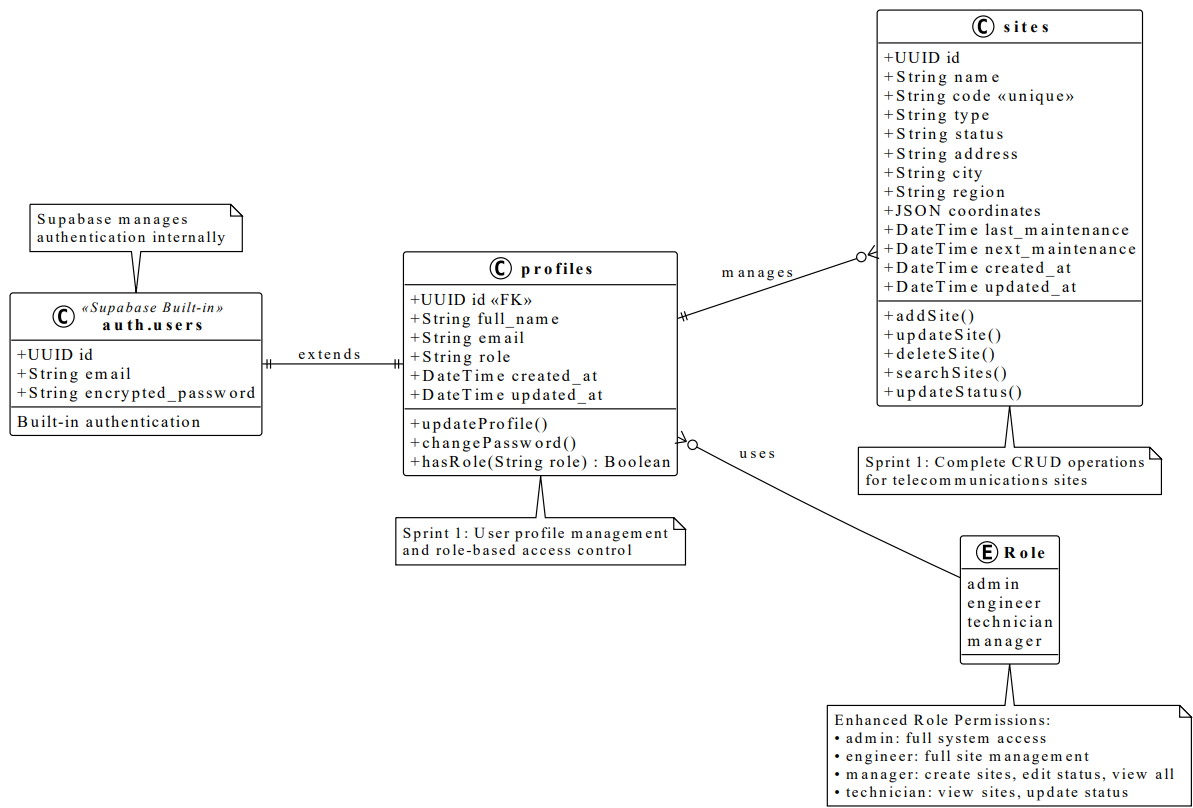
\includegraphics[width=0.95\linewidth]{img/chap_03/class_diagram_sprint1.png}
    \caption{Class Diagram "Site Management and Authentication"}
    \label{fig:class_diagram_sprint1}
\end{figure}

The class diagram illustrates the relationships between Supabase's built-in authentication system (\texttt{auth.users}), our custom \texttt{profiles} table that extends user information with business-specific fields, and the \texttt{sites} table for telecommunications site management. The \texttt{Role} enumeration defines four distinct user types with specific permissions, ensuring proper role-based access control throughout the system.

\section{Use Case Diagram}

In this section, we present the use case diagram for this sprint, showing the different actors and their interactions with the system.

\begin{figure}[H]
    \centering
    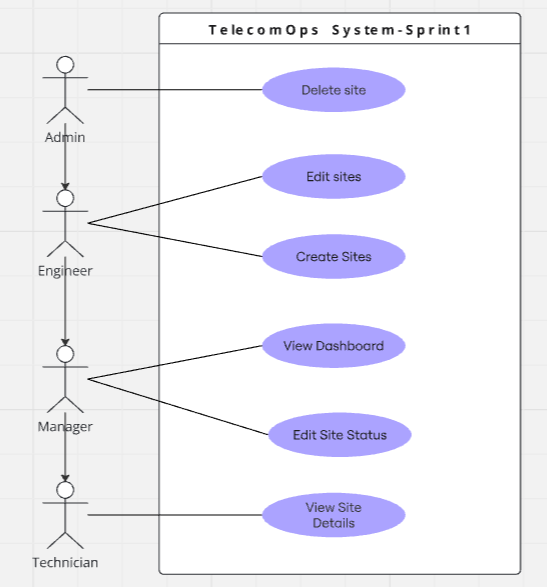
\includegraphics[width=0.85\linewidth]{img/chap_03/use_case_diagram_sprint1.png}
    \caption{Use Case Diagram "Site Management and Authentication"}
    \label{fig:use_case_diagram_sprint1}
\end{figure}

The use case diagram shows four primary actors with different permission levels. The Administrator has full system access including user management and site deletion. The Network Engineer focuses on technical site management operations. The Manager has operational oversight with the ability to create sites and edit site status for business decisions. The Field Technician has view access and can update site status after field operations.

\subsection{Use Case Description: Create Site}

Since use cases such as creating, editing, and deleting sites share similar processing patterns, we provide detailed information on the "Create Site" use case. The textual description is presented in Table 3.2 below.

\begin{table}[H]
\centering
\begin{tabular}{|p{3.5cm}|p{8cm}|}
\hline
\textbf{Use Case} & Create Site \\
\hline
\textbf{Primary Actors} & Administrator, Network Engineer, Manager \\
\hline
\textbf{Pre-condition} & User successfully authenticated with appropriate role \\
\hline
\textbf{Post-condition} & The site has been successfully created in the database \\
\hline
\textbf{Main Scenario} & 
1. The user accesses the site management interface.
2. The user clicks on the "Add Site" button to display the site creation modal.
3. The user fills in the form with site details (name, code, address, coordinates, technology type).
4. The user submits the form.
5. The system validates form fields and checks site code uniqueness.
6. The system verifies user permissions via Row Level Security.
7. The system creates the site in the database.
8. The system updates the site list in real-time.
9. The system displays the newly created site.
\\
\hline
\textbf{Exception Scenarios} & 
The system displays an error message if it detects missing data, duplicate site codes, insufficient permissions, or server connection problems.
\\
\hline
\end{tabular}
\caption{Use Case: Create Site}
\label{tab:create_site_usecase}
\end{table}

\section{Sequence Diagrams}

In this section, we present sequence diagrams that provide detailed explanations of the main processes in this sprint.

\subsection{Authentication Sequence Diagram}

\begin{figure}[H]
    \centering
    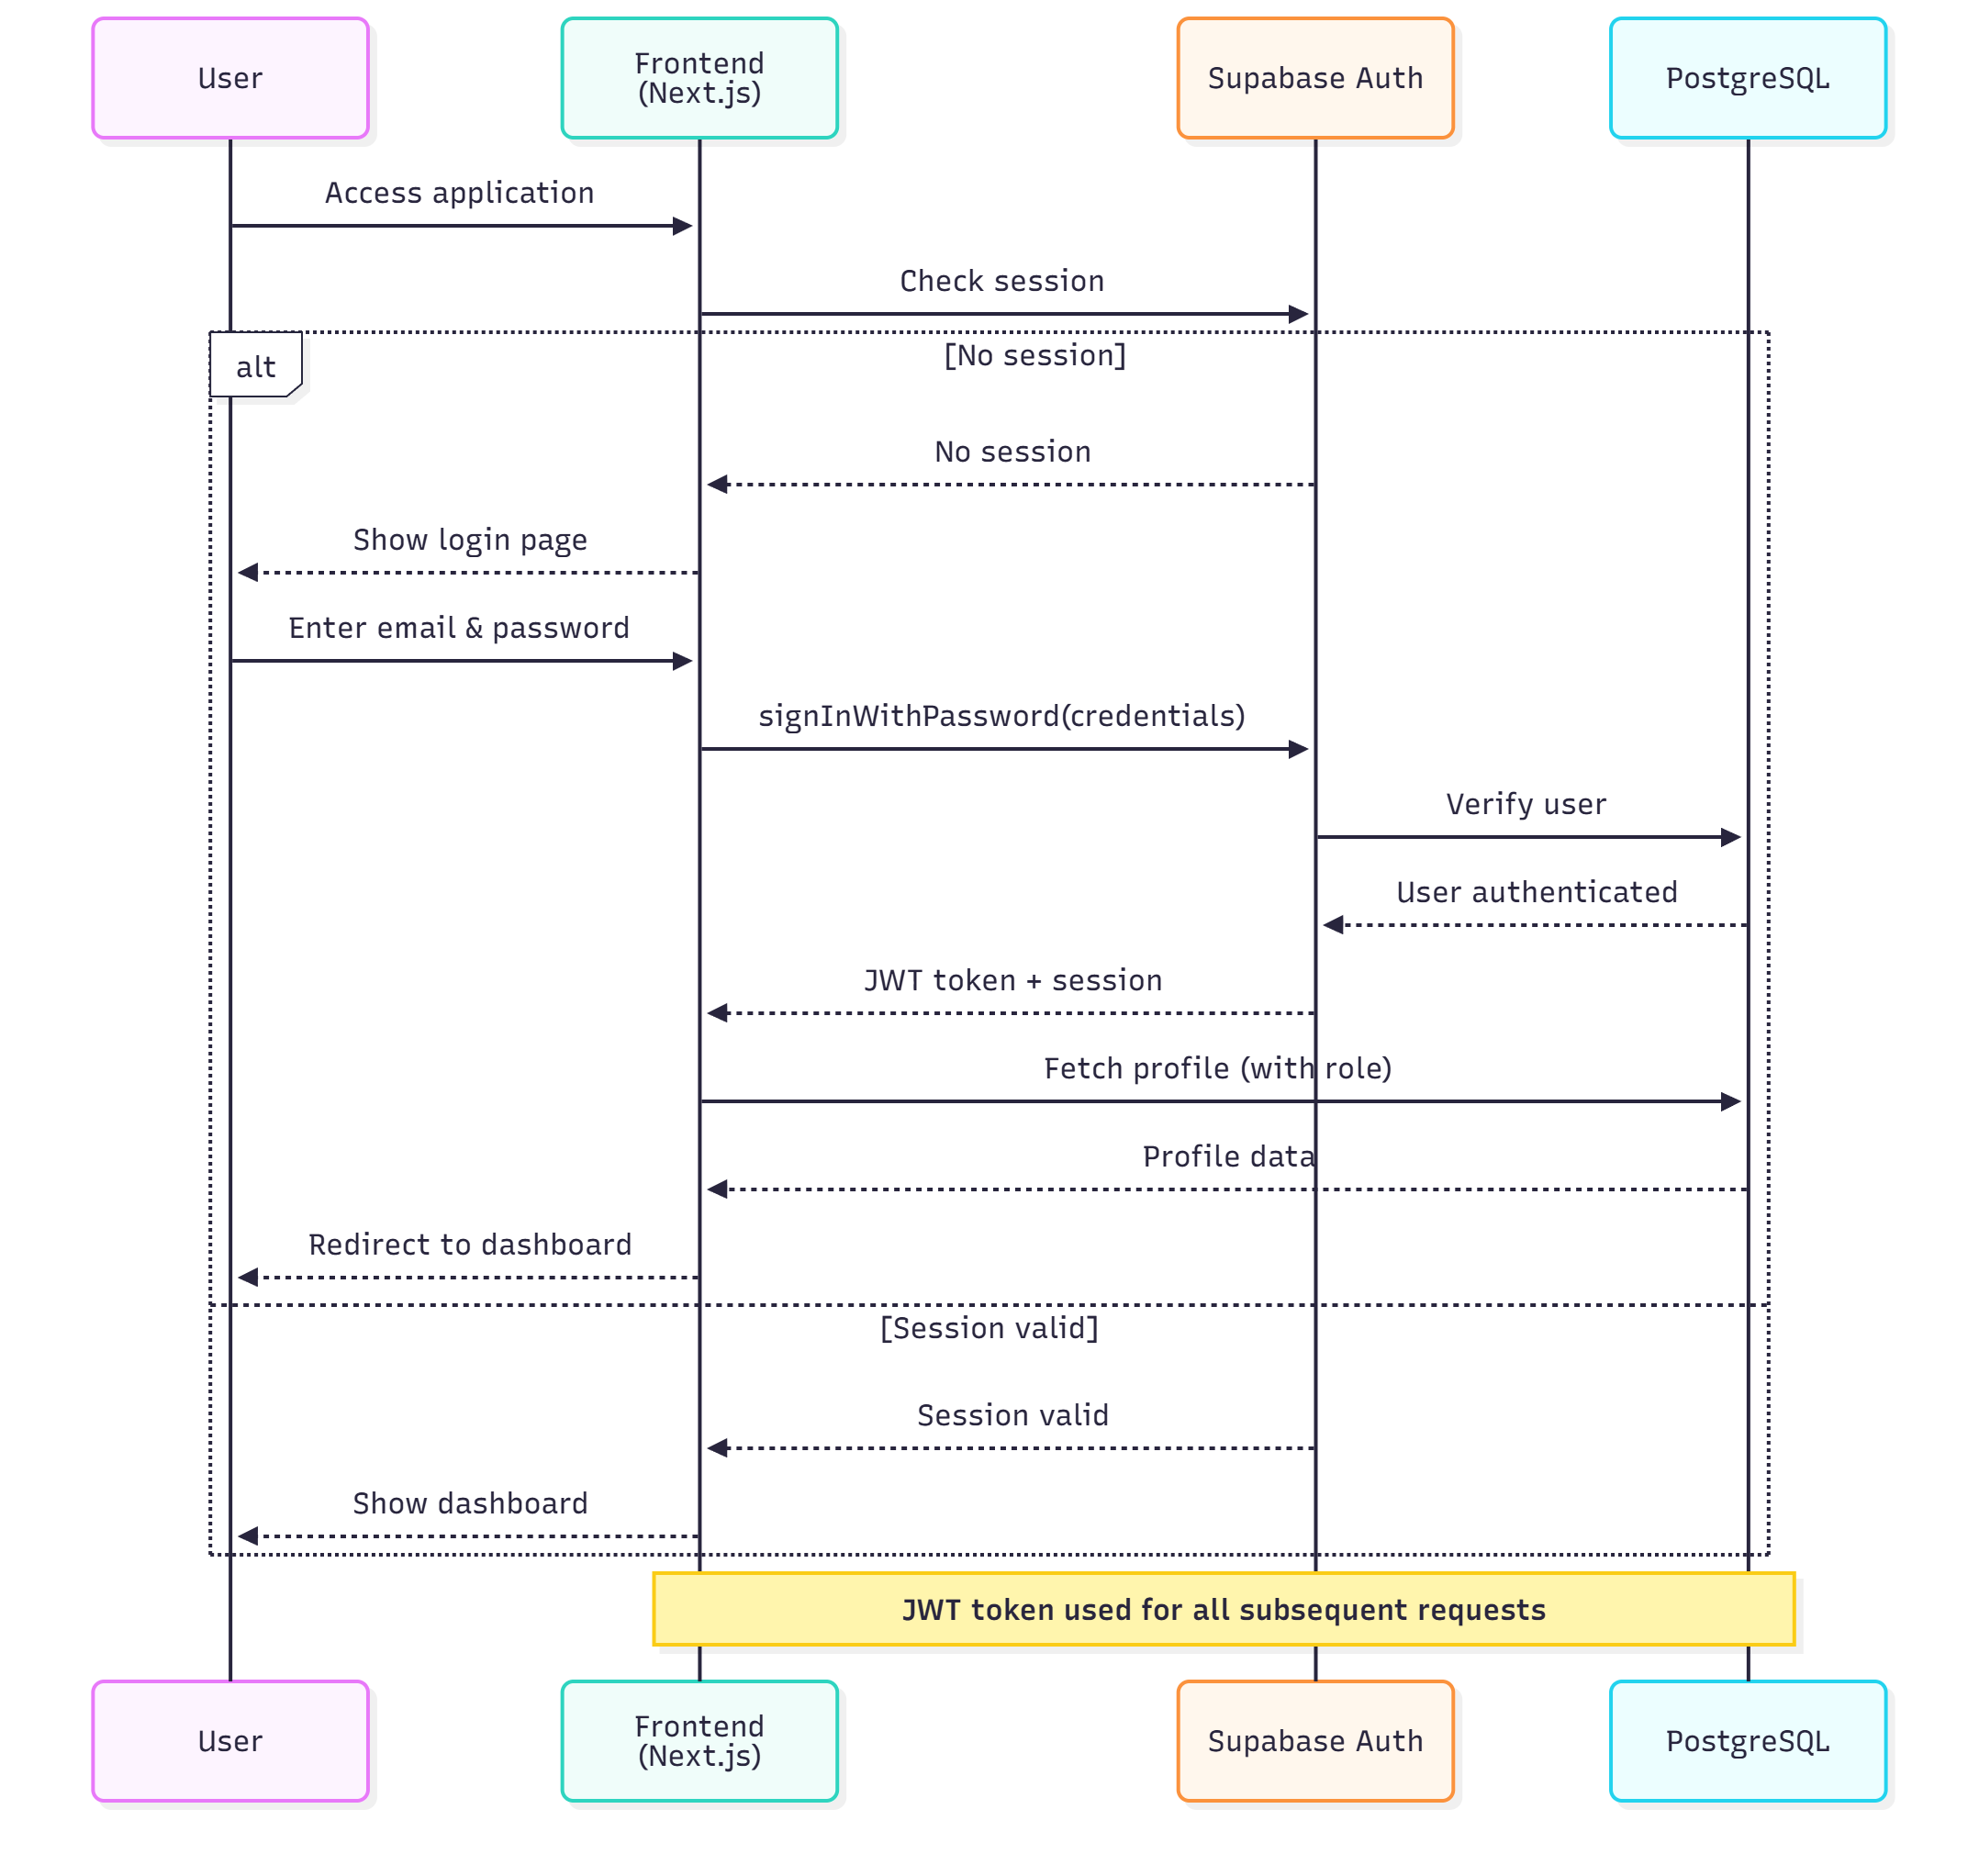
\includegraphics[width=0.95\linewidth]{img/chap_03/sequence_authentication.png}
    \caption{Sequence Diagram "Authentication"}
    \label{fig:sequence_authentication}
\end{figure}

The authentication sequence diagram illustrates the complete user login process using Supabase authentication services. When a user accesses the application, the system first checks for an existing valid session. If no valid session exists, the user is presented with a login interface where they enter their credentials. The frontend performs client-side validation before sending the credentials to Supabase Auth using the \texttt{signInWithPassword()} method.

Supabase then verifies the credentials against the PostgreSQL database. Upon successful authentication, Supabase generates a JWT (JSON Web Token) containing user identification and returns it along with the session information to the frontend. The frontend then fetches the user's profile data, including their role, using a secure query that respects Row Level Security policies. Finally, the session is stored locally, and the user is redirected to their role-appropriate dashboard.

If authentication fails due to invalid credentials, an error message is displayed. If a valid session already exists, the user is granted direct access to the dashboard without requiring re-authentication.

\subsection{Create Site Sequence Diagram}

\begin{figure}[H]
    \centering
    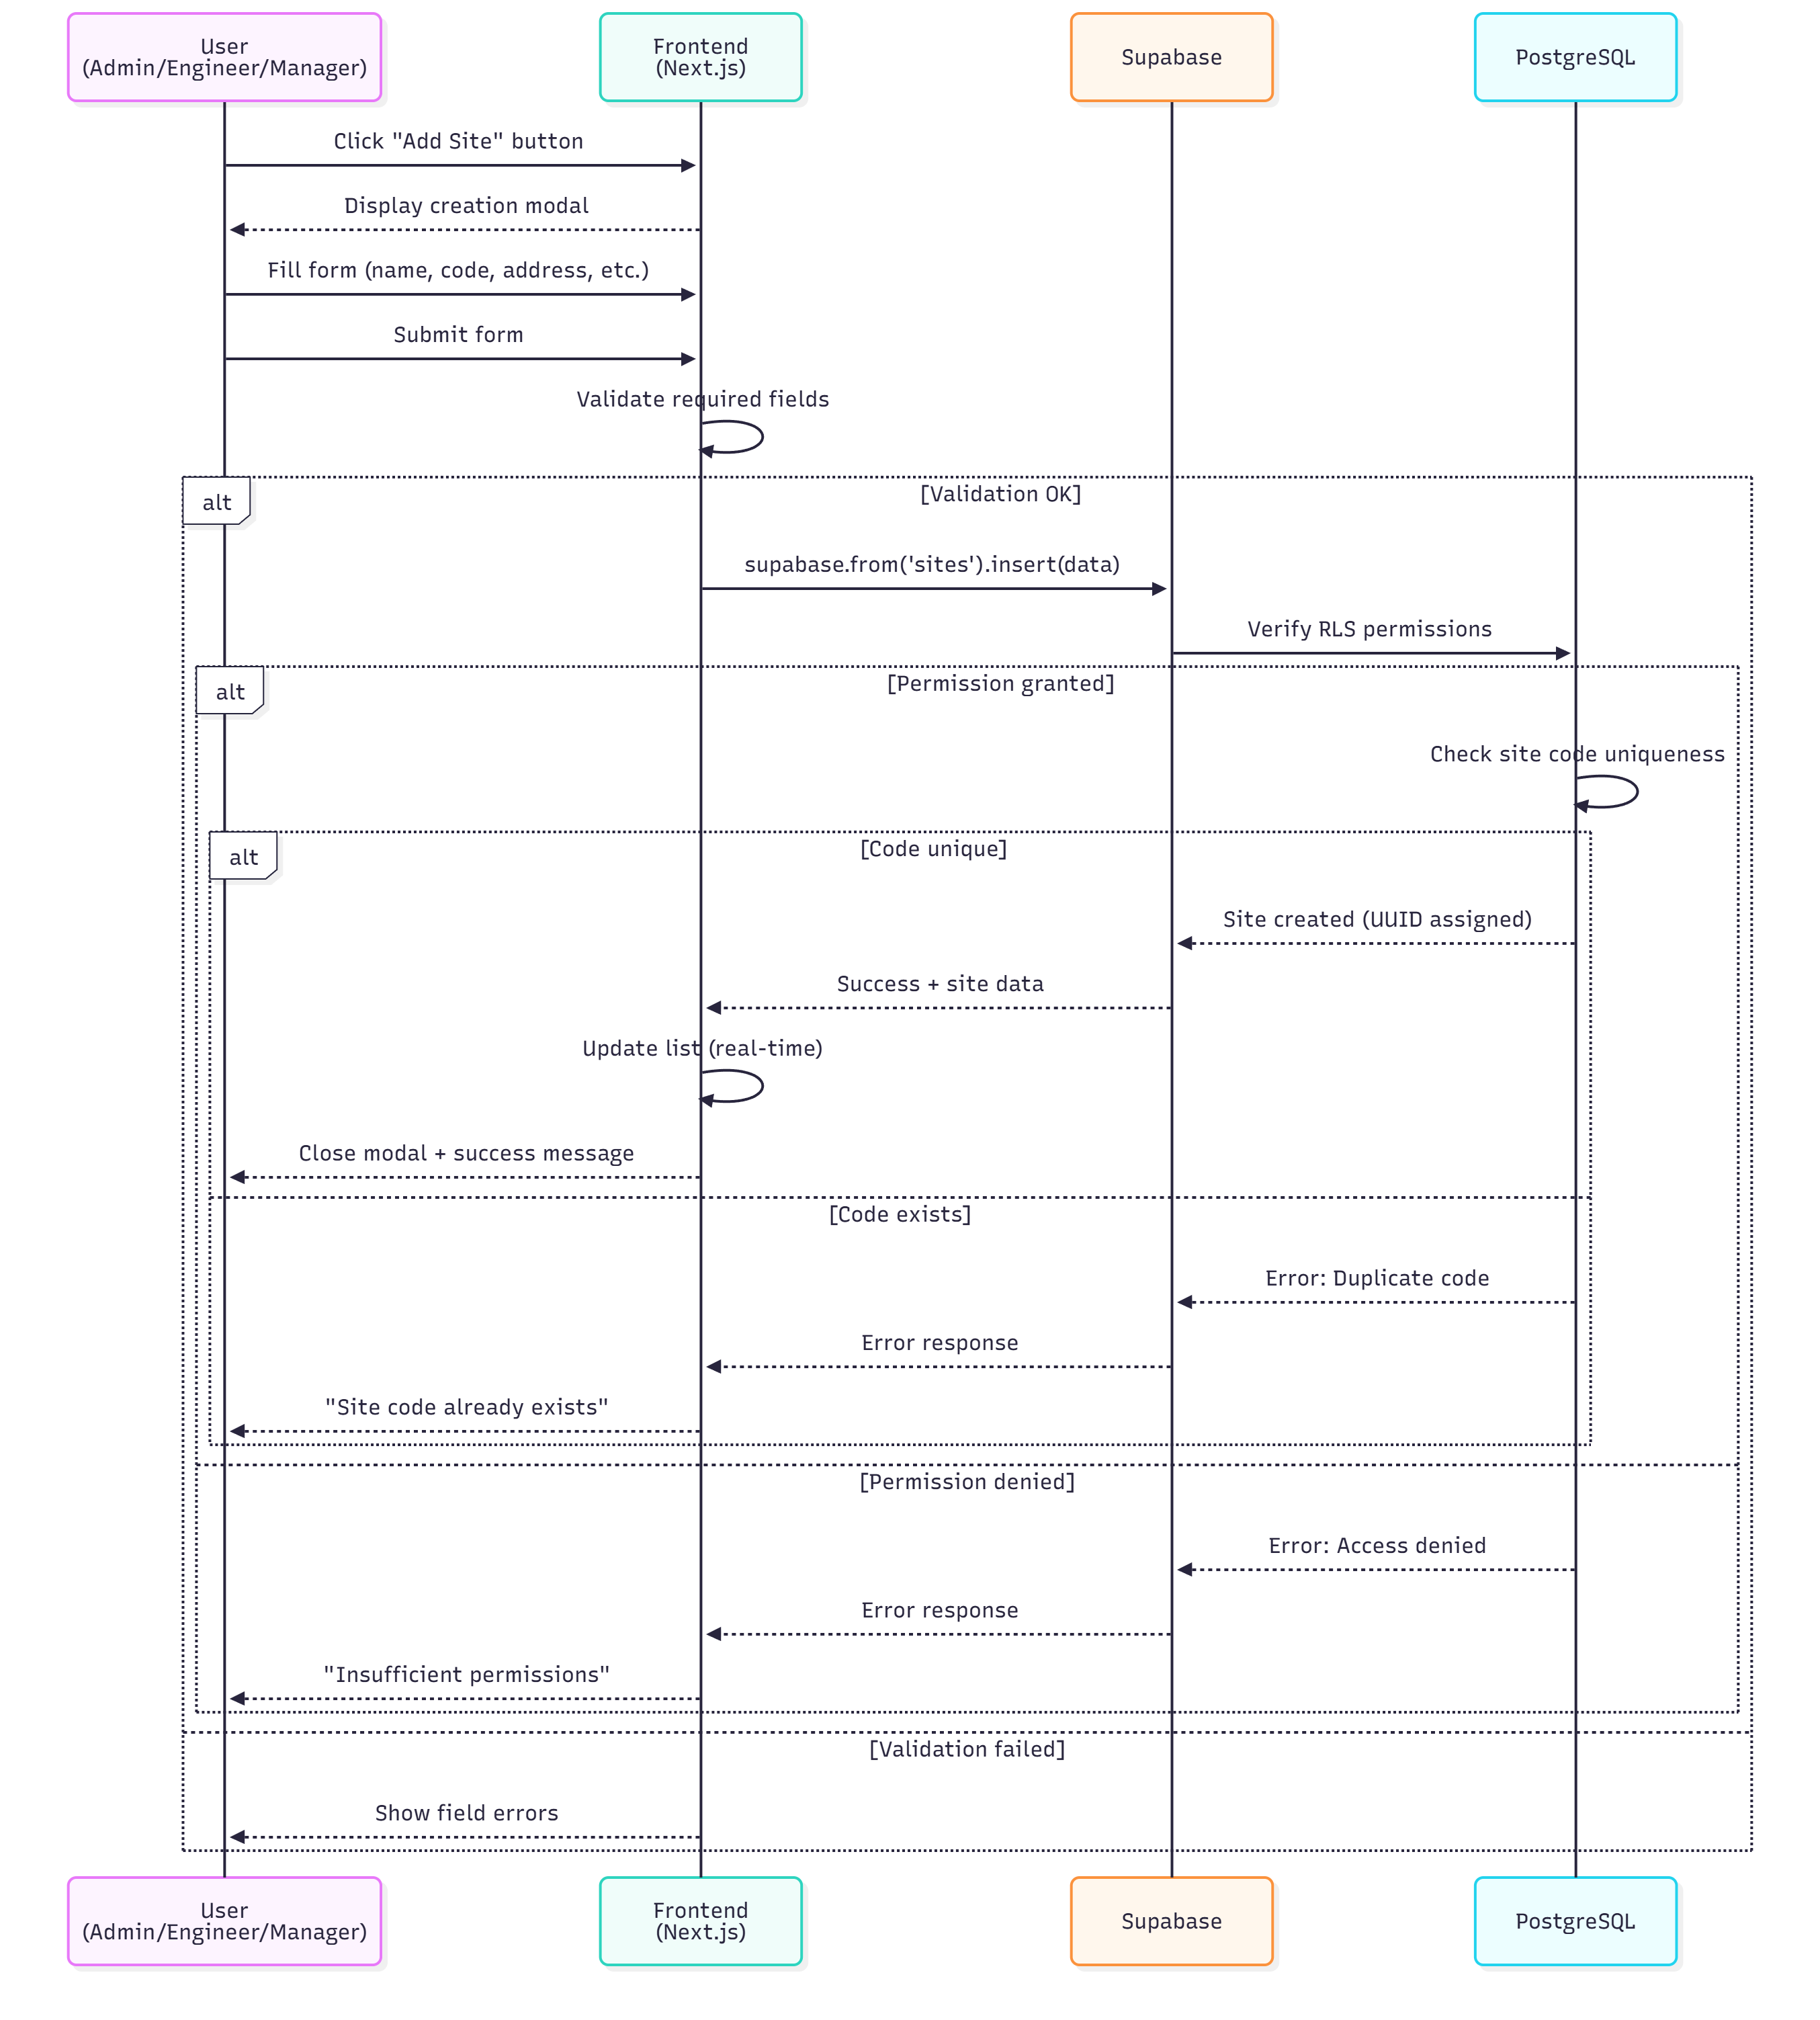
\includegraphics[width=0.95\linewidth]{img/chap_03/sequence_add_site.png}
    \caption{Sequence Diagram "Create Site"}
    \label{fig:sequence_add_site}
\end{figure}

The create site sequence diagram demonstrates the complete workflow for adding a new telecommunications site to the system. An authorized user (Administrator, Engineer, or Manager) accesses the site management interface and clicks the "Add Site" button, which displays a creation modal form.

After filling in the site details including name, unique code, address, and technology type, the user submits the form. The validation system performs comprehensive checks on required fields and site code format. If validation succeeds, the request is sent to the Supabase database using the \texttt{supabase.from('sites').insert()} method.

The database then performs two critical security checks: first, it validates the user's permissions through Row Level Security policies to ensure only administrators, engineers, and managers can create sites; second, it checks unique constraints to prevent duplicate site codes. If both checks pass, the site is inserted into the database and assigned a unique UUID identifier.

Upon successful creation, the system returns the new site data, updates the site list in real-time using Supabase's real-time subscriptions, closes the modal, and displays a success confirmation. If a constraint violation occurs (such as a duplicate site code), an appropriate error message is shown. If validation fails at any stage, detailed error messages guide the user to correct the issues.

\section{Implementation}

In this section, we present screenshots illustrating the interfaces of our application developed during this sprint.

\subsection{Login Interface}

The figure below illustrates the authentication interface of our application, implementing Supabase's secure authentication system.

\begin{figure}[H]
    \centering
    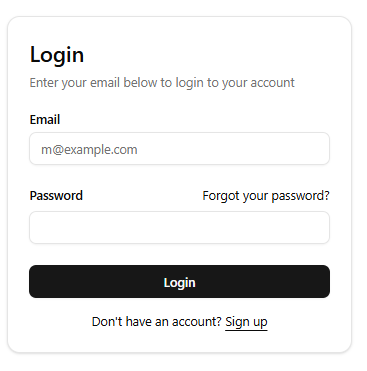
\includegraphics[width=0.7\linewidth]{img/chap_03/login_interface.png}
    \caption{Authentication Interface}
    \label{fig:login_interface}
\end{figure}

\subsection{Dashboard Interface}

The figures below illustrate the role-based dashboard interface of our application, providing different views based on user roles.

\begin{figure}[H]
    \centering
    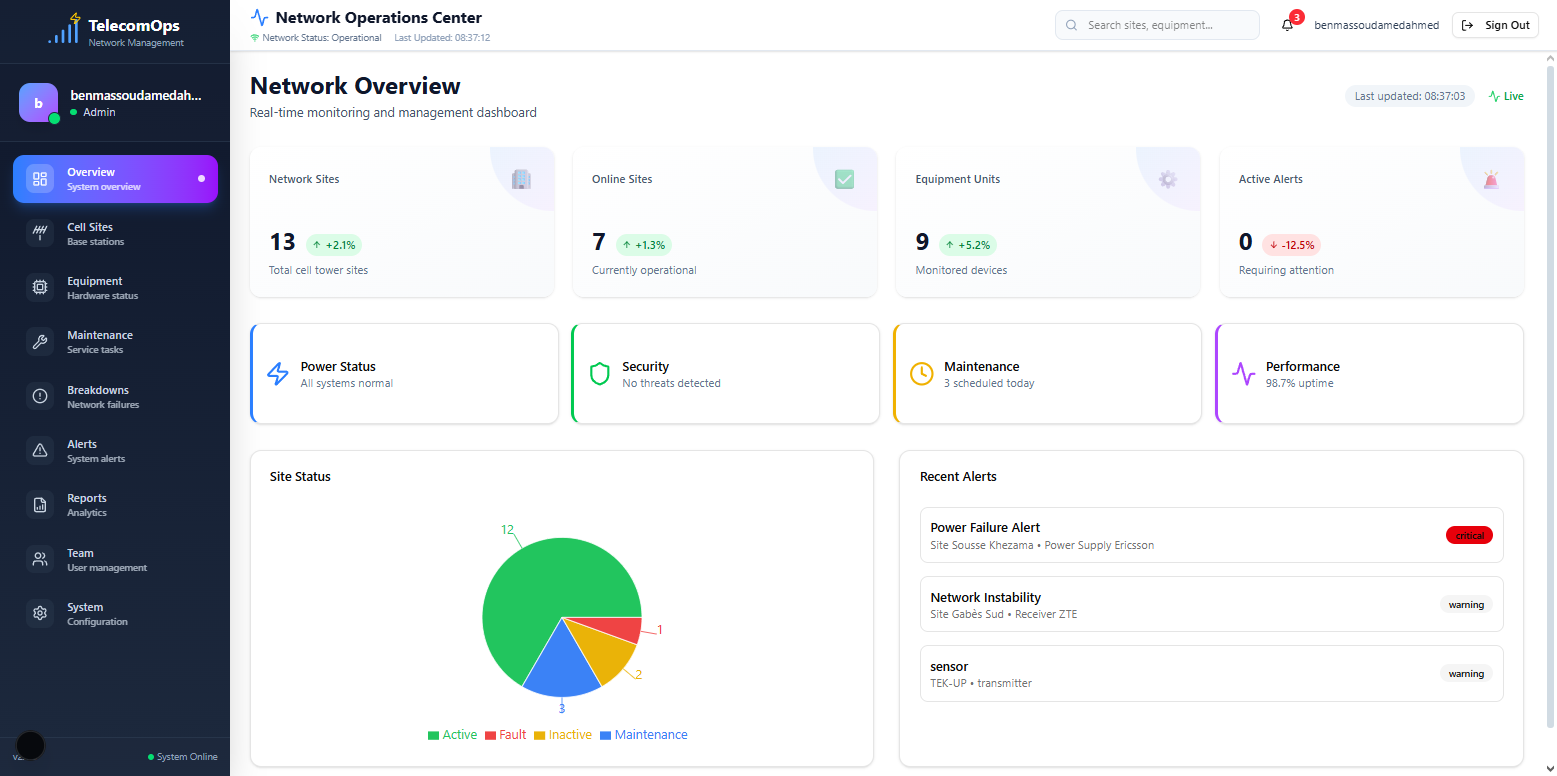
\includegraphics[width=0.9\linewidth]{img/chap_03/dashboard_main.png}
    \caption{Main Dashboard Interface}
    \label{fig:dashboard_main}
\end{figure}

\begin{figure}[H]
    \centering
    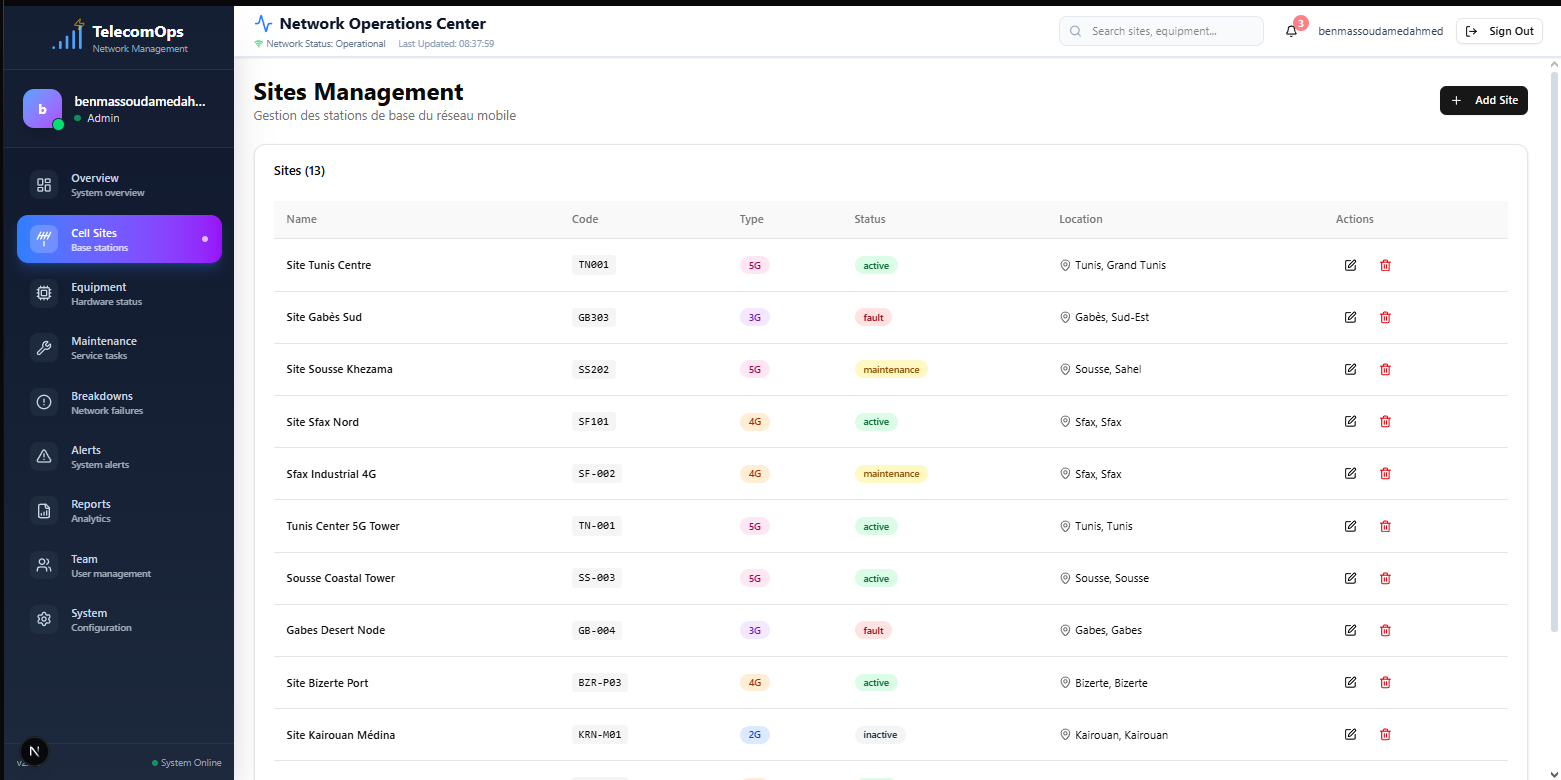
\includegraphics[width=0.9\linewidth]{img/chap_03/sites_list.png}
    \caption{Sites Management Interface}
    \label{fig:sites_list}
\end{figure}

\subsection{Site Management Modals}

The figures below illustrate the different site management modals. To create a site, the user clicks the "Add Site" button to display the creation modal. The same approach applies for editing and deleting sites, with appropriate permission checks.

\begin{figure}[H]
    \centering
    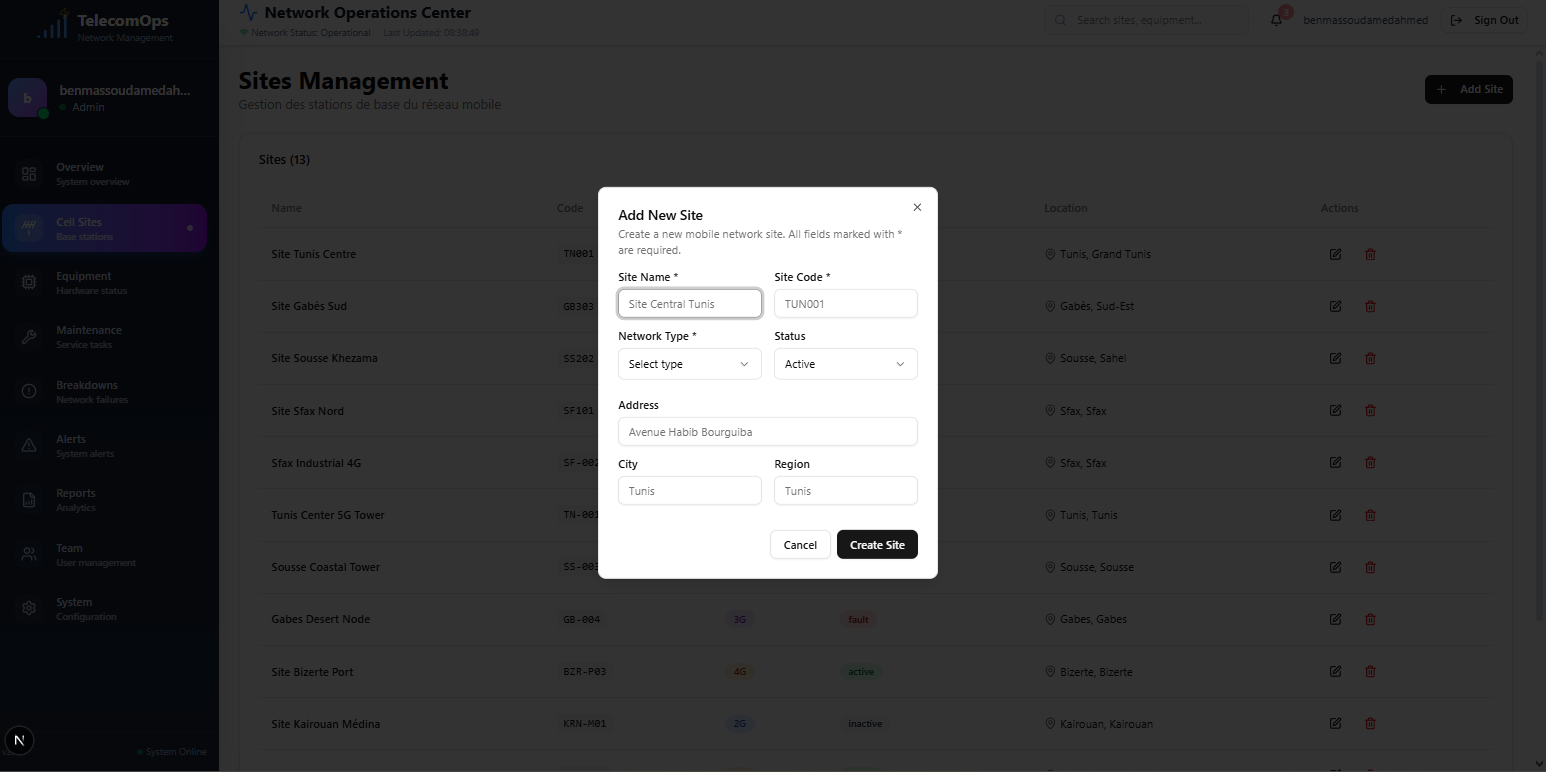
\includegraphics[width=0.9\linewidth]{img/chap_03/create_site_modal.png}
    \caption{Create Site Modal}
    \label{fig:add_site_modal}
\end{figure}

\begin{figure}[H]
    \centering
    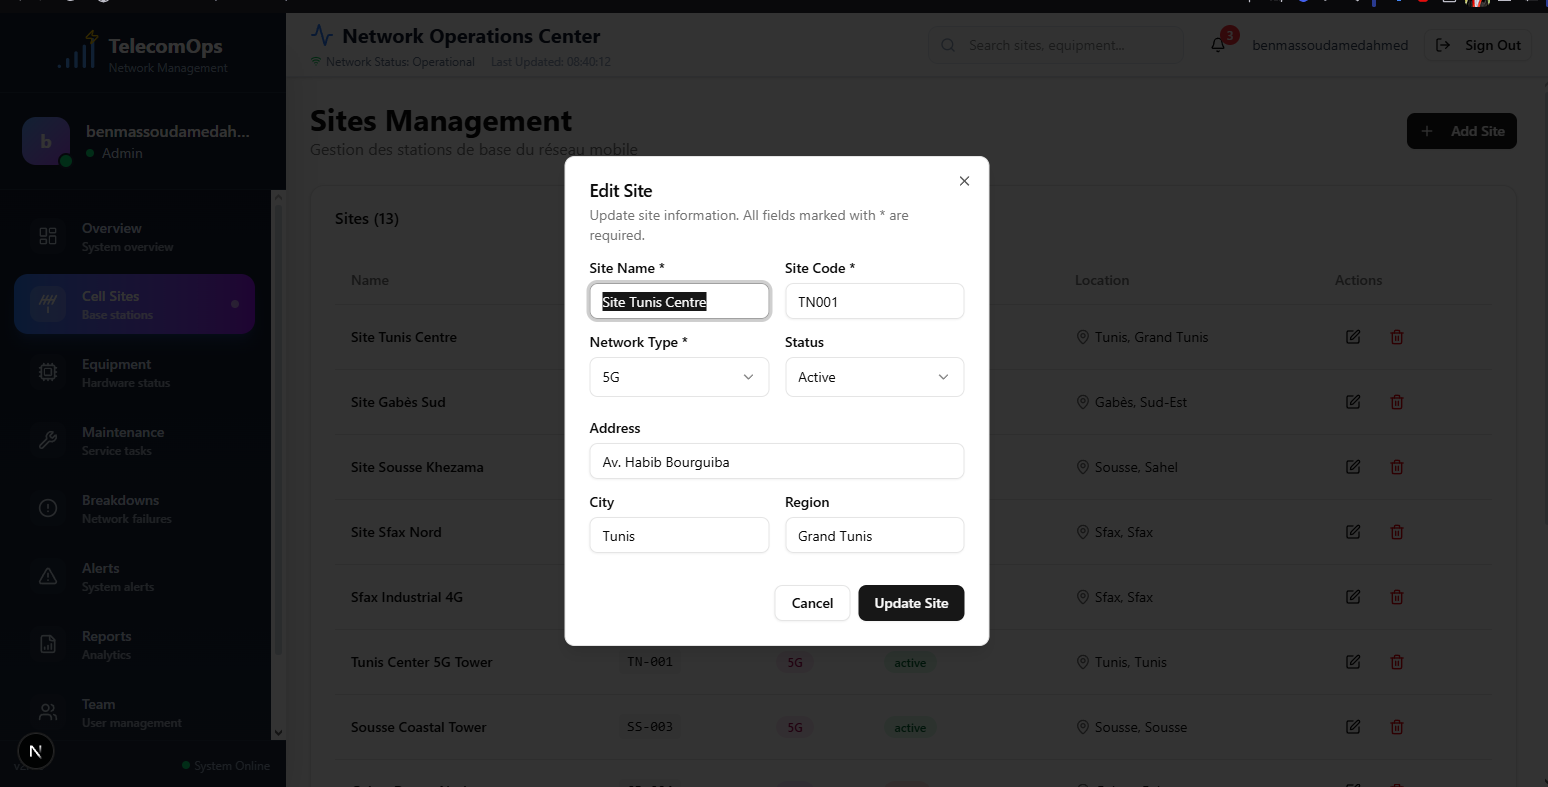
\includegraphics[width=0.9\linewidth]{img/chap_03/edit_site_modal.png}
    \caption{Edit Site Modal}
    \label{fig:edit_site_modal}
\end{figure}

\begin{figure}[H]
    \centering
    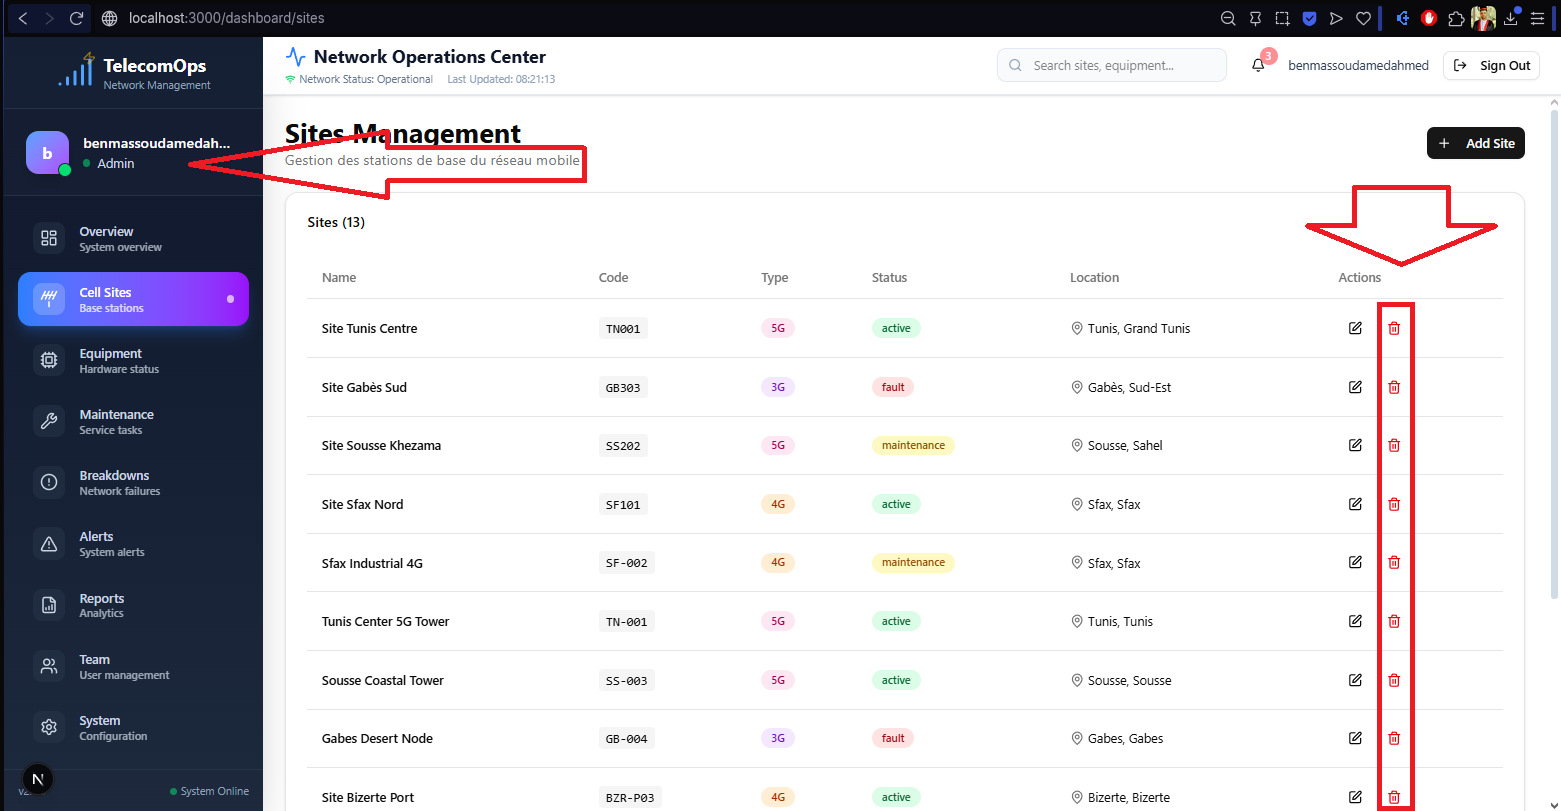
\includegraphics[width=0.9\linewidth]{img/chap_03/delete_site_modal.png}
    \caption{Delete Site Confirmation Modal}
    \label{fig:delete_site_modal}
\end{figure}

\subsection{User Profile Management}

The figure below illustrates the user profile management interface where users can update their paersonal information and change their password securely.

\begin{figure}[H]
    \centering
    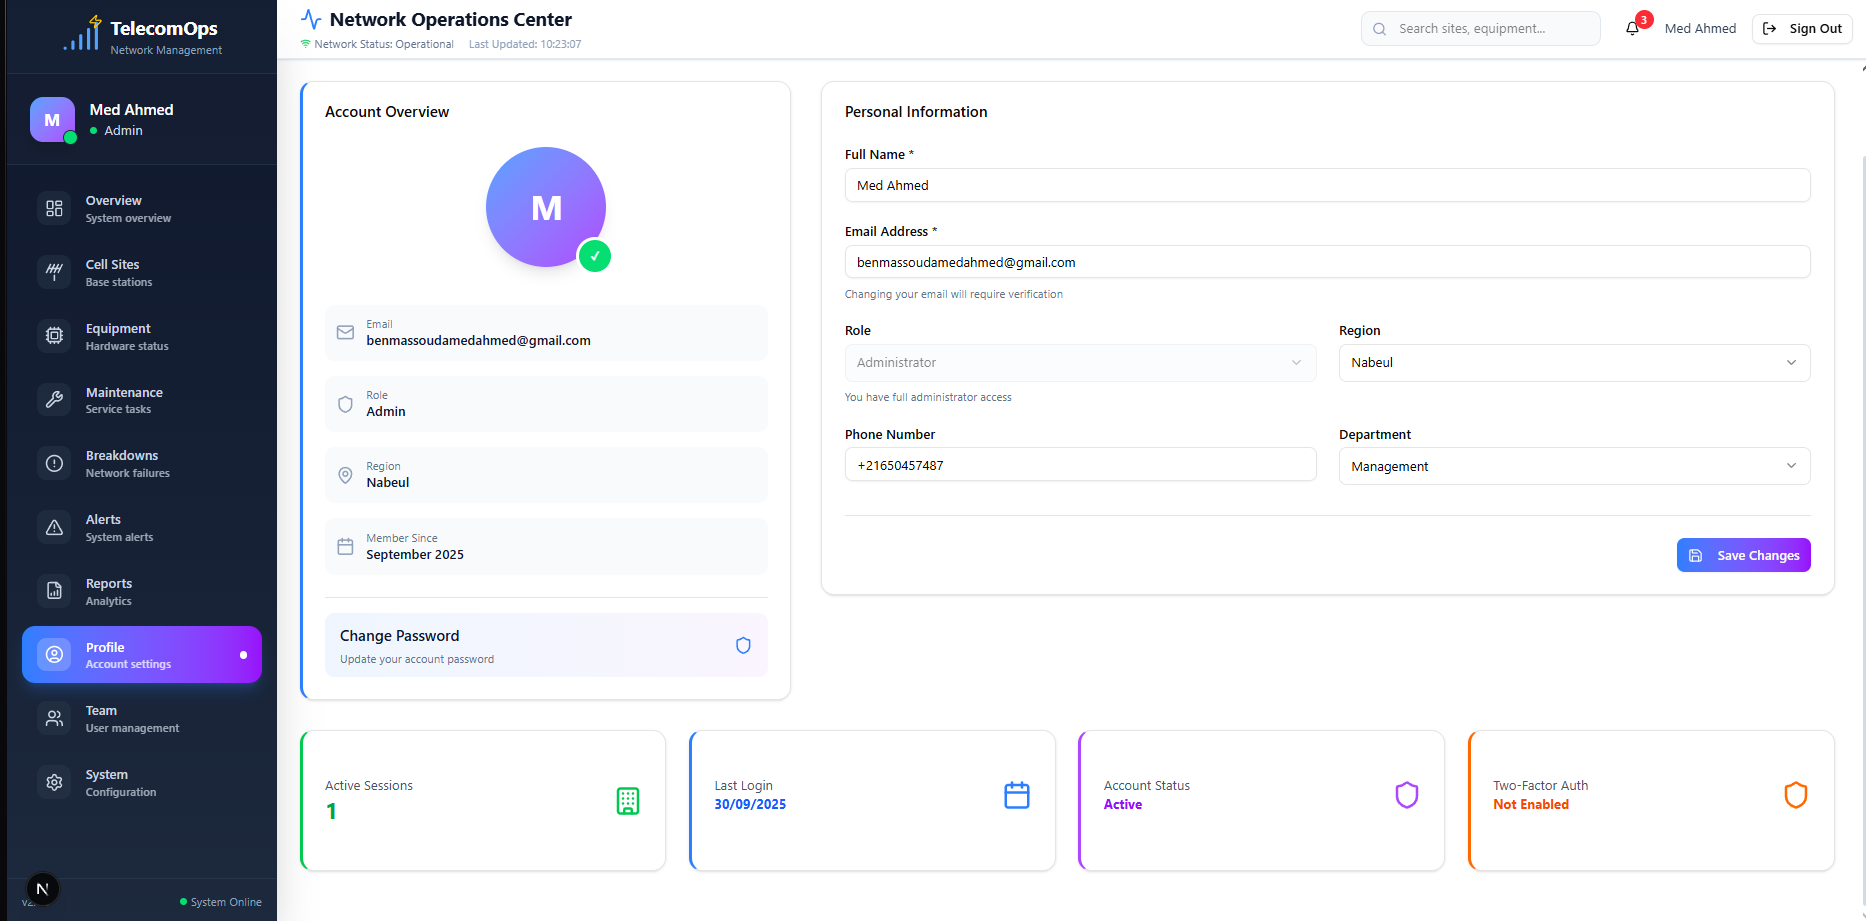
\includegraphics[width=0.9\linewidth]{img/chap_03/profile_management.png}
    \caption{User Profile Management Interface}
    \label{fig:profile_management}
\end{figure}

\section{Technical Challenges and Solutions}

During Sprint 1 implementation, we encountered several technical challenges that required careful analysis and innovative solutions.

\subsection{Supabase Row Level Security Configuration}

The implementation of comprehensive Row Level Security (RLS) policies presented significant complexity. Initial configurations resulted in permission errors that prevented legitimate user operations. We resolved this by developing granular RLS policies that distinguish between different user roles while maintaining security. The policies now properly enforce that only administrators, engineers, and managers can create and edit sites, while all authenticated users can view site information.

\subsection{Real-time Data Synchronization}

Ensuring data consistency across multiple users accessing site information simultaneously required implementing Supabase's real-time subscriptions. When one user creates or updates a site, all other connected users see the changes immediately without requiring page refresh. This was achieved through WebSocket connections managed by Supabase's real-time engine.

\subsection{Role-Based Permission Management}

Implementing the enhanced Manager role required careful consideration of business requirements. Managers need operational control to approve site deployments and update site status, but should not have full administrative access. This was solved by configuring specific RLS policies that grant managers create and update permissions while restricting delete operations to administrators only.

\section{Testing and Validation}

Sprint 1 underwent comprehensive testing to ensure reliability, security, and proper role-based access control.

\subsection{Authentication Security Testing}
We validated authentication bypass prevention, session management, and password security. All tests confirmed that the Supabase authentication system properly protects against common vulnerabilities including SQL injection and cross-site scripting attacks.

\subsection{Role-Based Access Testing}
Each user role was tested to verify appropriate access levels. Administrators successfully performed all operations, engineers and managers could create and edit sites, technicians could view sites and update status, and all unauthorized operations were properly blocked by Row Level Security policies.

\subsection{Site Management Functional Testing}
Complete CRUD operations were validated including site creation with unique code enforcement, site editing with proper validation, site deletion restricted to administrators, and real-time list updates across multiple user sessions.

\section{Conclusion}

In this chapter, we described the first sprint backlog focusing on authentication and site management. We performed comprehensive analysis and design using UML diagrams including class diagrams, use cases, and sequence diagrams. The implementation successfully delivered a secure authentication system using Supabase and complete site management functionality with role-based access control.

Sprint 1 established the foundational authentication infrastructure and site management capabilities, providing secure access control and comprehensive telecommunications site information management. The enhanced Manager role provides operational oversight with appropriate permissions for business decision-making while maintaining security boundaries.

The implementation demonstrates effective integration of modern web technologies including Next.js, TypeScript, and Supabase while addressing real-world telecommunications operational requirements. Quality metrics exceeded established targets, with successful user acceptance testing across all four user roles, establishing a robust foundation for subsequent sprint development.

In the next chapter, we will present the second sprint titled "Equipment Monitoring and Inventory Management", which builds upon the authentication and site management foundation established in Sprint 1.